\chapter{Background}
\section{OPC UA}
\subsection{Introduction}
In a proprietary system, connected devices may use different communication protocols. Software used to inspect and operate this system must be aware of all these protocols. 
This requires additional costs and time spent on creating and maintaining such a system. The complexity can be reduced by using the OPC UA standard for communication \cite{CPOpcTech}.

\subsection{Legacy OPC}
OPC is a data exchange standard for communication between multiple data sources. These sources may include factory devices, laboratory equipment, databases, and test system fixtures. A set of standard interfaces were defined by OPC Foundation to allow access to any device compatible with OPC \cite{whatopc}.

The first protocol is referred to as OPC Classic and it used Microsoft's COM(Component Object Model)/DCOM(Distributed Component Object Model) technology. 
COM/DCOM enabled communication between processes in multiple languages for Windows operating system. 
COM is an interface standard designed for software components and it allows systems to be built from different software vendors, that are designed to use this interface
COM is providing a communication interface layer, allowing both local and remote procedure calls between processes. 
Distributed COM (DCOM) is an extension of COM designed for distributed applications. DCOM allows components to communicate across the network.\cite{COMDCOM, intrOPC}.

The OPC Classic specifications provided definitions for accessing data, alarms, events, and historical data\cite{OPCCLas}:
\begin{itemize}
  \item OPC Data Access (DA) - exchange of data which includes values, time and quality information in real time,
  \item OPC Historical Data Access (HDA) - reading, updating, and subscribing to historical data and events,
  \item and OPC Alarms and Events (A\&E) - receiving alarms and responding to them, reveiving events.
\end{itemize}

Because it relies on the Microsoft Windows platform, OPC Classic has some limitations like security issues or dependency on Windows. \cite{whyOPC}

{  
  \color{red}
  OPC Implementation? - jest to calkiem fajnie opisane w \cite{intrOPC}, ale nie wiem czy doda� bo mozliwe ze by�by to zbyt duzy offtop, bo uzywam opc ua.
}
\subsection{OPC UA}
In 2006 OPC Foundation released OPC Unified Architecture (UA) which is an improvement on OPC Classic. It brings together all the different specifications of OPC Classic into a single entry point with DA, A\&E with HDA of both.

\subsubsection{Communication impovements}
OPC UA is based on a cross-platform Service-Oriented Architecture (SOA). SOA is an improvement on the security and functionality that was in OPC Classic with Microsofts COM/DCOM technology.

OPC UA supports two protocols:
\begin{itemize}
  \item Binary protocol - requires minimal resources, easy passing through firewall
  \item Simple Object Access Protocol (SOAP) - uses HTTP/HTTPS ports
\end{itemize}

By using SOA and web services OPC UA became independent from Windows operating system. It means devices no longer had to be running Windows and OPC UA could be deployed on other operating systems, like Linux or Mac.\cite{whyOPC}

\subsubsection{Security imporovements}
Security in OPC UA was greatly improved by switching from COM/DCOM. OPC Classic used security features from DCOM, which were complex and difficult. This caused common oversights in that department and disabled the security options altogether.

To secure data, OPC UA uses common web technologies as a security basis, which includes authentication and encryption features. Clients and servers use certificates to connect. OPC UA supports PKCS12 Public-Key Cryptography Standards to supply the X.509 private keys and certificate files containing public keys. 
There are three possible messaging modes between the server and client:
\begin{itemize}
  \item None
  \item Sign
  \item Sign and Encrypt
\end{itemize}
User also has the ability to enable Basic256 or Basic128Rsa15 security policy, which are bases for signing and encrypting the data.\cite{whyOPC}

\subsection{OPC UA Specification}
Specifications of OPC UA are split into parts, also known as IEC 62541 standards. The specifications parts are divided between core specifications, which establish the base for OPC UA, and access type specific elements, which specify information models. An overview showing these specifications is presented in the figure \ref{fig:opc-ua-spec}.

\begin{figure}[ht]
  \centering
  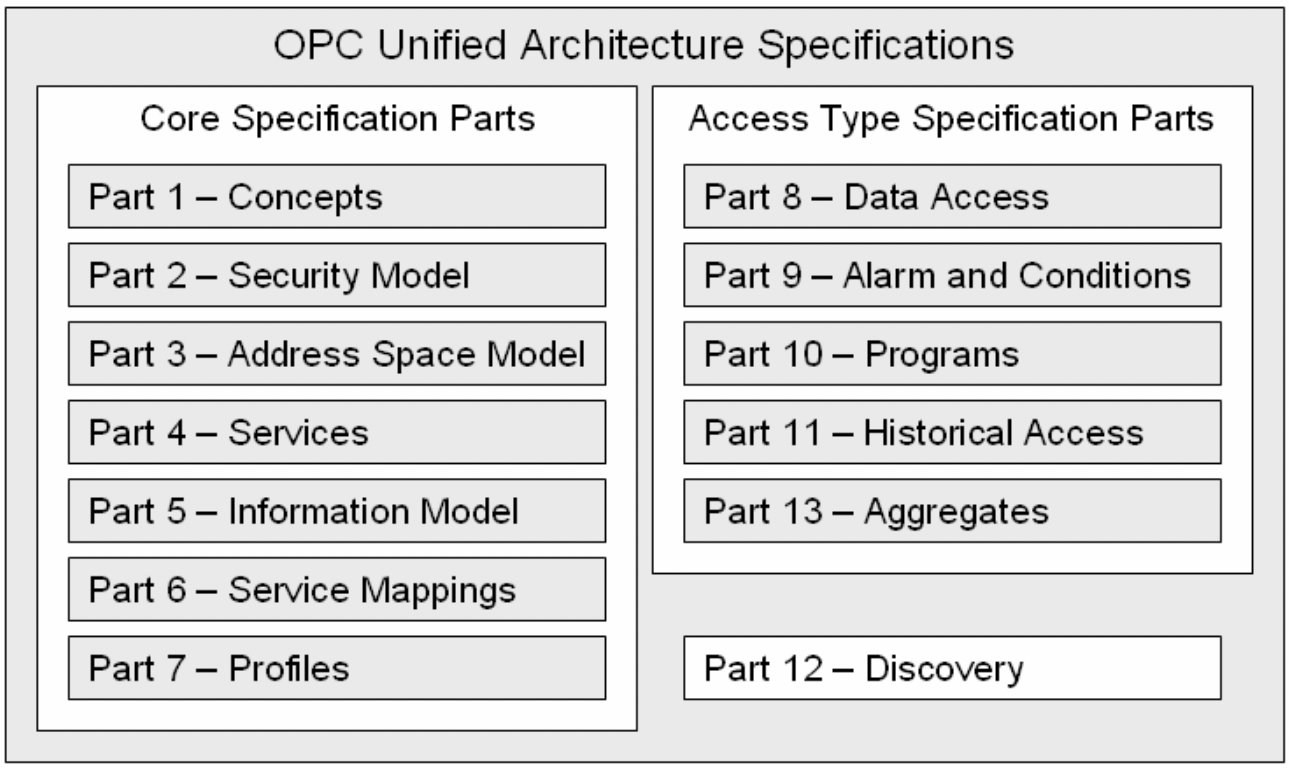
\includegraphics[width=0.7\linewidth]{figures02/opc-ua-specifications.png}
  \caption{OPC UA Specifications \cite{Damm2009OPCUA}}
  \label{fig:opc-ua-spec}
\end{figure}

\subsubsection{Core specification parts}
The concepts in part 1 provide an overview of OPC UA, and the security requirements and model are described in part 2. 

The specifications that are crucial to understanding how to model and access information are parts 3 and part 4. 

The Address Space Model in part 3 specifies the model used to define and expose information models, as well as to create an OPC UA address space. 

The possible relations between OPC UA client and server applications are represented in abstract UA Services in part 4. Client applications use Services to get information from the server. The services are not defined as a concrete representation of communication used by an application, but they define the information to be exchanged.

Part 6 explains how the UA Services are mapped to messages, how security methods are applied to them, and how the messages are wired. 

Part 5 contains the base information model, which is used to create information models that use OPC UA. This specification part defines:
\begin{itemize}
  \item The entry points into the address space that clients use to navigate through the instances and types of an OPC UA server
  \item The base types that serve as the foundation for the various type hierarchies
  \item The built-in but extensible types such as object types and data types
  \item The Server Object that provides capability and diagnostic information
\end{itemize}

The profiles in part 7 are used to define subsets of OPC UA features to implement by an UA application to provide interoperability for such subsets. Two levels of subsets are defined in the specification:
\begin{itemize}
  \item Conformance Units - first level, defines a small set of functionality that is used together and can be tested and verified
  \item Profiles - second level, list of conformance units
\end{itemize}

\subsubsection{Access type specification parts}

Part 8 includes the Data Access information model, which defines the representation and usage of automation data and specific characteristics.
Process alarm and condition monitoring are specified in the Alarms and Conditions information model defined in part 9.
Part 10 contains the Programs information model that defines a base state machine. 
The Historical Access information model describes the usage of history access Services and the presentation of information in part 11.
In part 13 the Aggregates specifies the computation of aggregated values from data samples.

\subsubsection{Discovery part}

The Discovery specifies how to discover servers in the network and how to get the necessary information needed for connection from a client in part 12.\cite{Damm2009OPCUA}


\subsection{OPC UA software layers}
OPC UA uses the client-server concept for communication. The UA server application exposes its information to other applications and the UA client is an application that consumes that information. An application might serve both as a UA server and client.

OPC UA is most often created from three software layers, as shown in \ref{fig:opc-ua-layers}. Here there is presented that the whole software stack can be implemented in Java, C/C++, or in .NET, but it is also possible to implement it in javascript, as in this thesis.

\begin{figure}[ht]
  \centering
  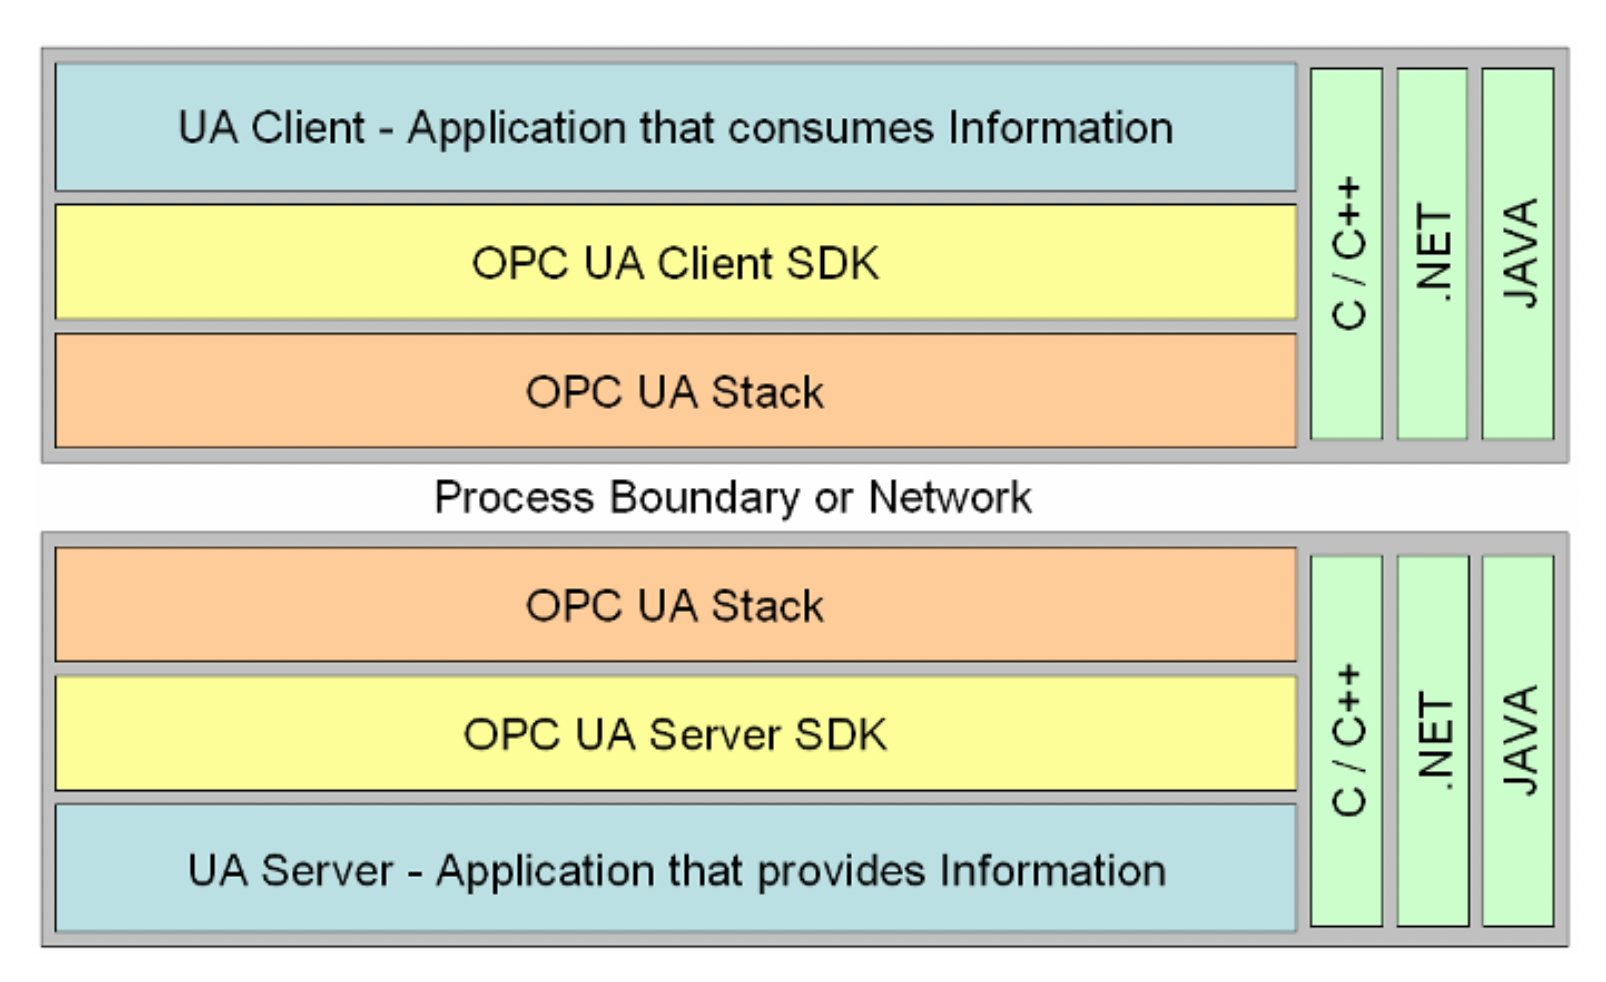
\includegraphics[width=0.7\linewidth]{figures02/opc-ua-layers.png}
  \caption{OPC UA software layers \cite{Damm2009OPCUA}}
  \label{fig:opc-ua-layers}
\end{figure}

OPC UA Application is a system that exposes or consumes information through OPC UA. OPC UA client or server SDK contains OPC UA functionalities, and UA Stacks implement communication channels. \cite{Damm2009OPCUA}

\subsubsection{Information Modeling}
\subsubsection{}
\subsubsection{}
\subsubsection{}
%- TODO Cross-Platform Capabilities
%- TODO Expanded security?
%? TODO IT Integration
%? TODO Compatibility
% TODO applications
%TODO architecture
% TODO client
% TODO server
%TODO specification



{
\color{red}
OPC Unified Architecture
by Mahnke, Wolfgang, Leitner, Stefan-Helmut, Damm, Matthias
14.2.2 Is Information Modeling a Pain?
\url{ https://www.itk.ntnu.no/fag/TTK4545/TTK2/PDF/Extract%20from%20Book%20OPC%20Unified%20Architecture.pdf}
  
  https://www.ni.com/pl-pl/innovations/white-papers/12/why-opc-ua-matters.html\\
}

\section{Abstraction layers}
\subsection{Introduction}
Systems created currently are constructed using numerous abstraction layers. Each layer is defining an inteface that hides details of implementation for its functionality. Programs that are built on top of each layer can be used and understood using only its inteface, so it's not necessary to know the layer implementation.
\subsection{Specification}
Important aspect of an abstraction layer is its specification. A specification should capture the functionality of the implementation as well as the assuptions about other layer context. However, abstraction layers are not commonly specified and verified.
\subsection{Issues}
{
  \color{red}
  Write something about issues when creating abstraction layers\\
  
  sources: \\
  Deep Specifications and Certified Abstraction Layers \\
  http://flint.cs.yale.edu/flint/publications/dscal.pdf\\
  
  Separation Logic: A Logic for Shared Mutable Data Structures \\
  https://sci-hub.se/10.1109/LICS.2002.1029817\\
  https://ieeexplore.ieee.org/document/1029817\\
  
  Theories of Programming Languages\\
  John C. Reynolds\\
  
  Clean code\\
  str 36, 93, 290\\
}